

\subsection{Grafiken und Animationen}

\begin{figure}[H]
    \centering
    \label{fig:mine_exterior_concept}
    \caption{Concept Art -> Finale Grafik}
    \subfloat[][]{\fbox{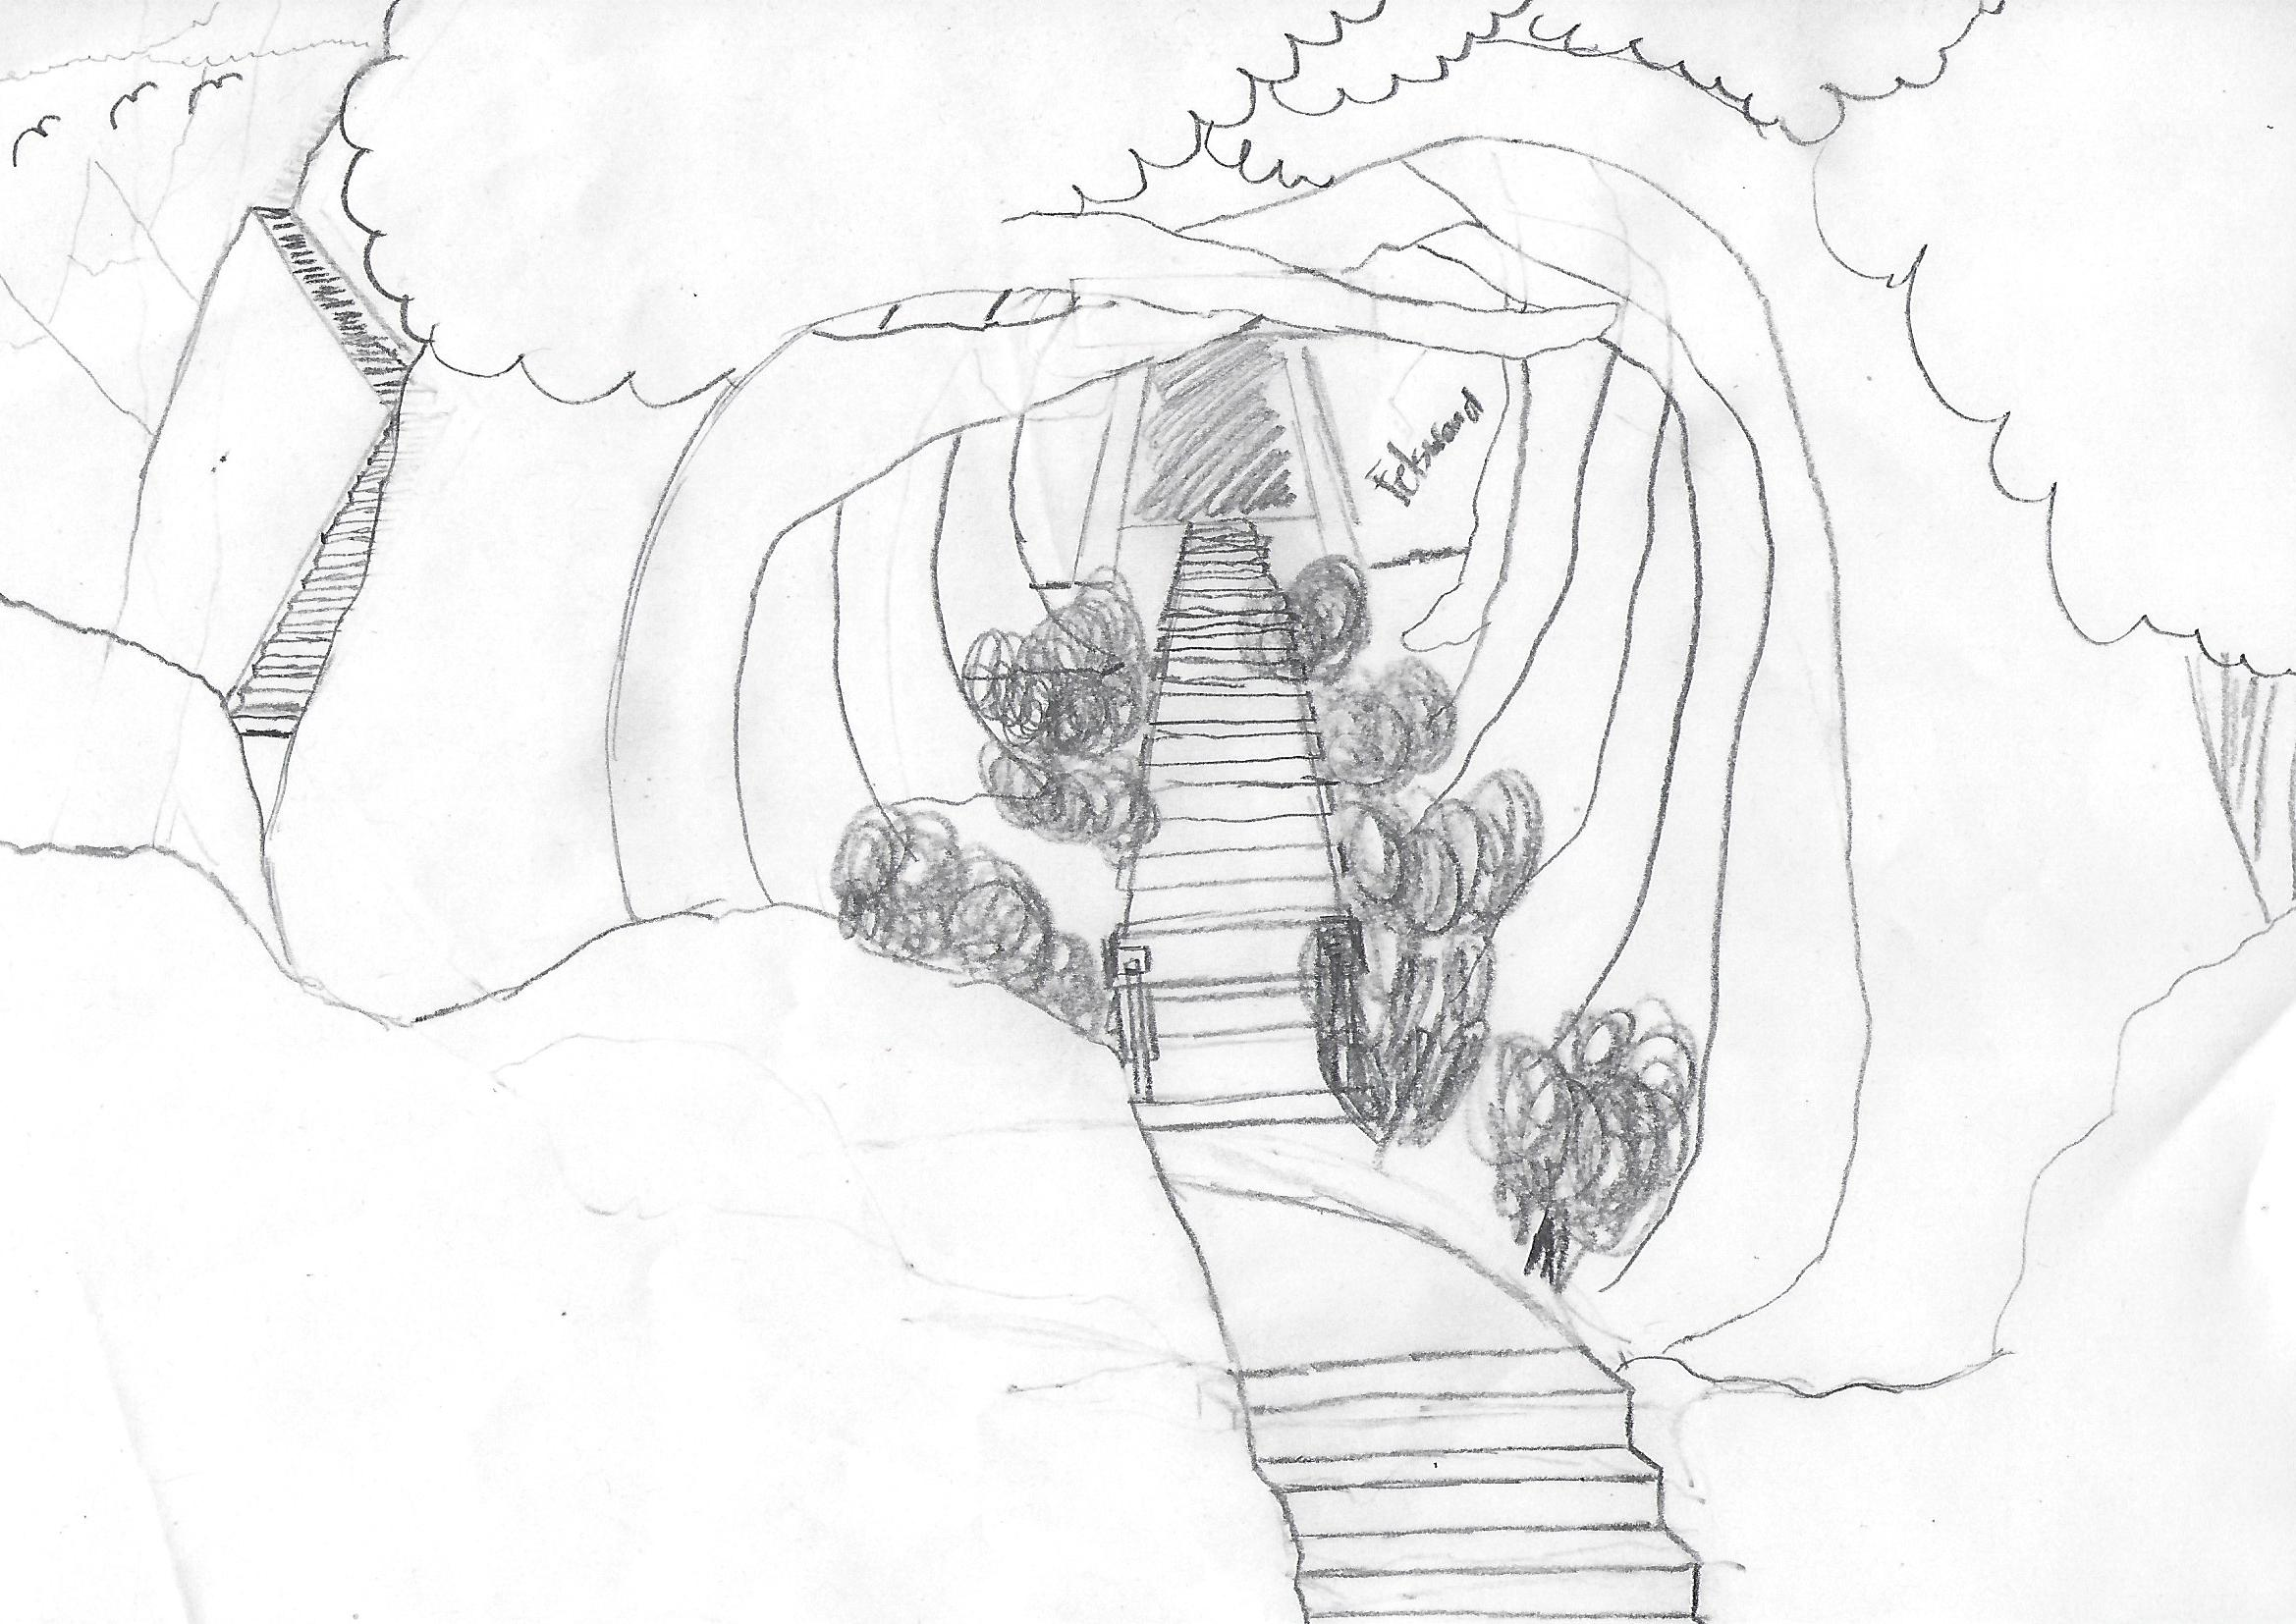
\includegraphics[width=0.5\linewidth]{mine_exterior_concept}}}
    \subfloat[][]{\fbox{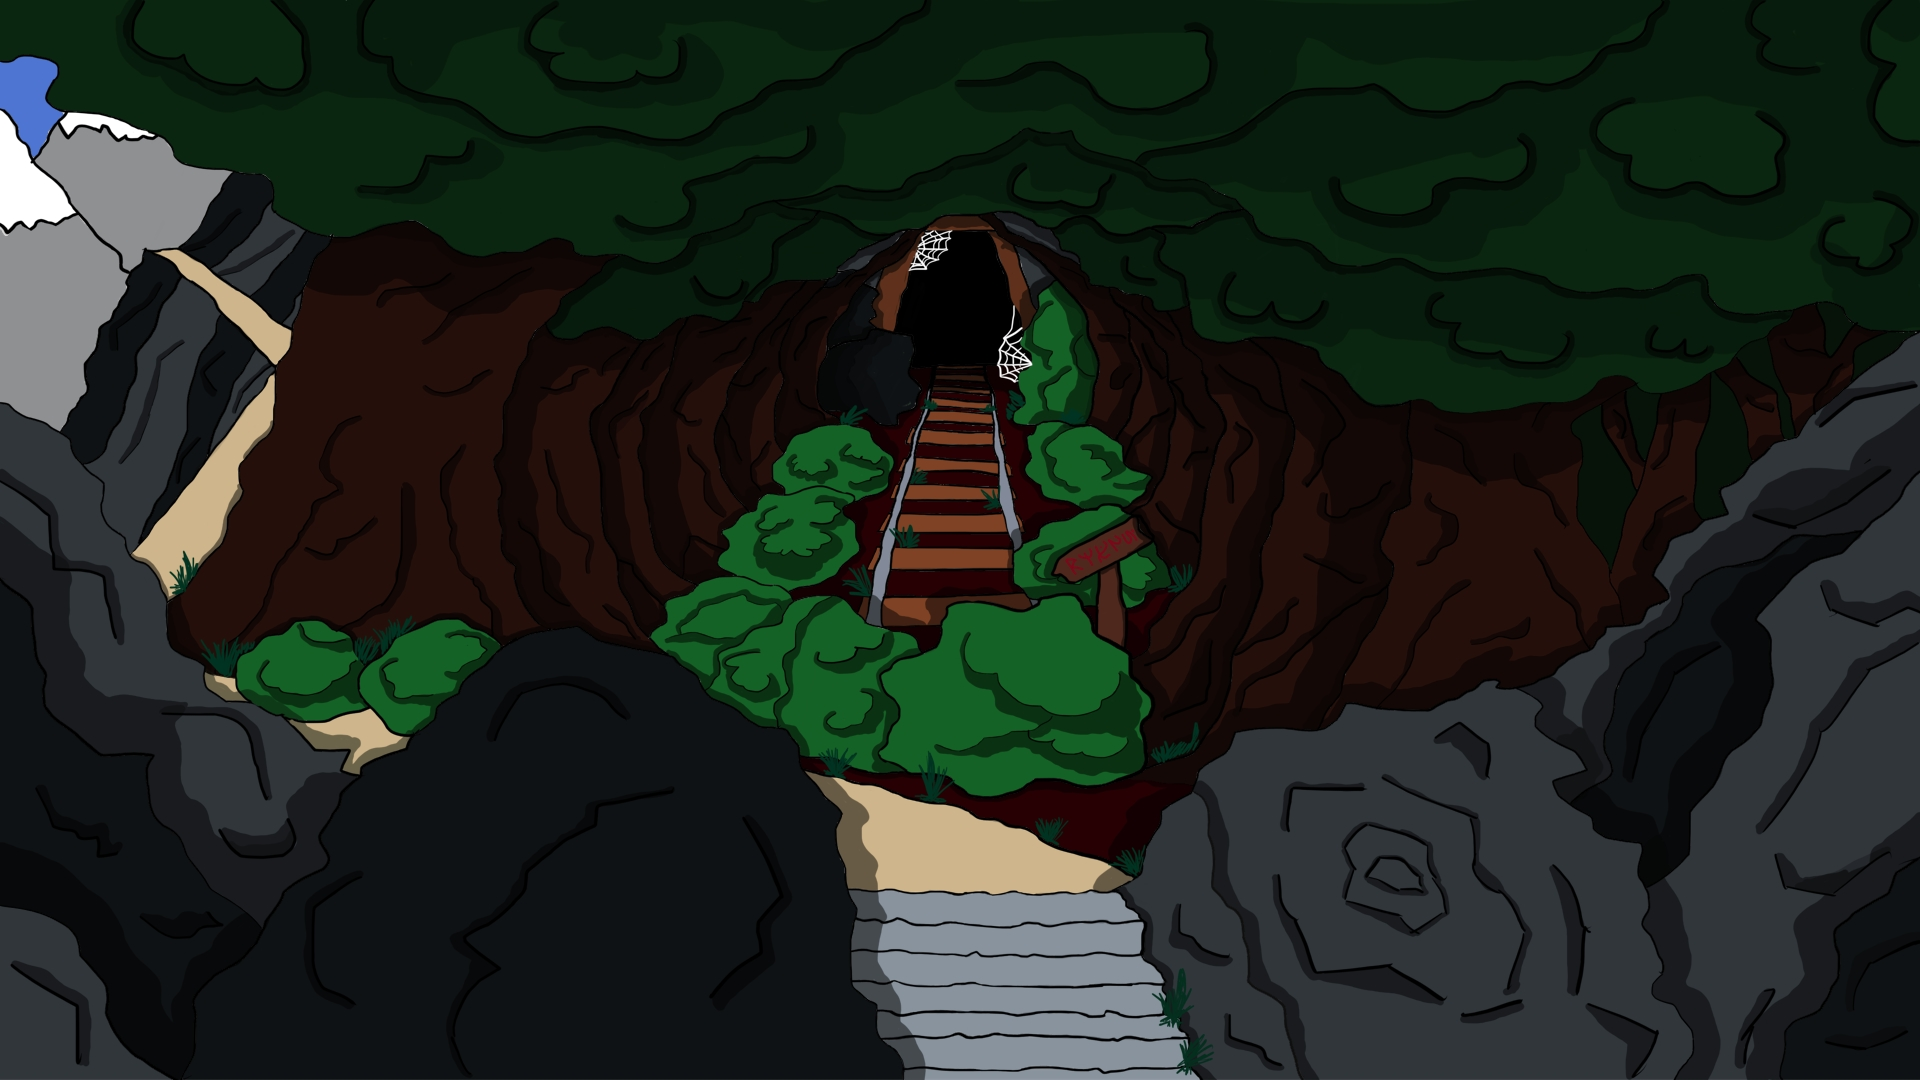
\includegraphics[width=0.5\linewidth]{mine_exterior_final}}}
\end{figure}

- Vorstellung Krita
    - kurz gehalten, Main Features --> Grafik der Oberfläche

- Digital Art
    - Inhaltliches:
        - Konzept:
            - Welche Grafik-Assets werden benötigt
            - Grafikstil
            - Animationen
        
        - Herausforderungen: 
            - zeitlicher Aufwand 
            - generell Zeichentechniken
            - tatsächlich benötigte Assets oft erst spät bekannt bzw. während Entwicklung neu hinzugekommen (z.B. SVG-Grafiken für Map)
    
    - Technisches:
        - Layer
        - Animationen
        - Dateitypen und -größen


\subsection{Frontend-Design}
    - Design
        - Stil (8-Bit Ära RPG/Adventure)
        - CSS Framework
        - Aufbau des Frontends (HTML-Seiten)
        - Design der einzelnen Seiten 

    - Technisches
        - Worldmap Areas -> SVG-Grafiken
        - 